% 2008 年四川卷理科第 19 题：平面 ABEF ⊥ 平面 ABCD，两个直角梯形 ABEF、ABCD，
%   ∠BAD = ∠FAB = 90°，BC ∥= ½AD，BE ∥= ½AF。
% 来源 PDF：gaokaomath-src/普通高考/2008/2008四川理.pdf
% SHA-256：dd251cfc43d7be2f75e2675f8bd73e8569900c65a53724312a95b1cec79a3a9b
% 原页：2008四川理.pdf 第 1 页（A3 三栏）第 3 栏，书页码 483。
% 重绘依据：与文科卷第 19 题同一几何体（理卷无 G、H），投影 (x,y,z)->(x+0.8y, 0.5y+z)。
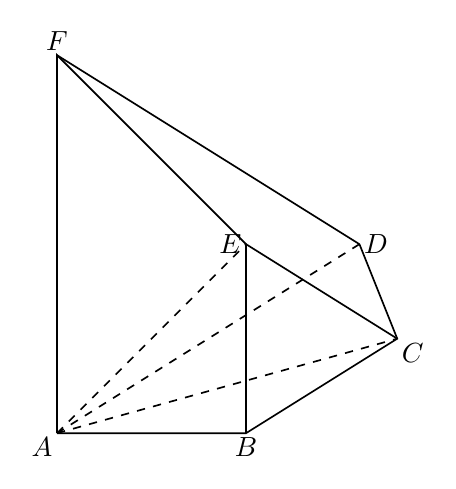
\begin{tikzpicture}[scale=1.2, semithick, every node/.style={inner sep=1.4pt}]
  \coordinate (A) at (0.00,0.00);
  \coordinate (B) at (2.00,0.00);
  \coordinate (C) at (3.60,1.00);
  \coordinate (D) at (3.20,2.00);
  \coordinate (F) at (0.00,4.00);
  \coordinate (E) at (2.00,2.00);

  % 底面 ABCD
  \draw (A) -- (B) -- (C) -- (D);
  \draw[dashed] (D) -- (A);
  \draw[dashed] (A) -- (C);

  % 立面 ABEF
  \draw (A) -- (F) -- (E) -- (B);

  % 侧棱与内部虚线
  \draw (C) -- (E);
  \draw (D) -- (F);
  \draw[dashed] (A) -- (E);

  \node[below left] at (A) {$A$};
  \node[below] at (B) {$B$};
  \node[below right] at (C) {$C$};
  \node[right] at (D) {$D$};
  \node[above] at (F) {$F$};
  \node[left] at (E) {$E$};
\end{tikzpicture}
